The tracking sub-detectors are responsible for registering spacial coordinates of charged particles.
The coordinates from multiple layers of tracking sub-systems are processed by the tracking algorithms
to produce {\it tracks}, which are objects representing the trajectory of a charged particle. There are
three distinct tracking sub-detectors in \lhcb shown in \figref{lhcb_detector_cross_section}; Closest to the interaction point is
the {\it VErtex LOcator}, \velo, then just before the \lhcb magnet is the {\it Tracking Turisensis}, \ttracker,
and  lastly the {\it Outer Tracker} \ot. There are several track types that are {\it reconstructed} by
the tracking algorithms, depending on which of the tracking sub-detectors provided information to produce
the track object. The varius track types are shown in \figref{}. The most common tracks used are {\it long}
which have the highest momentum resolution. The overal reconstruction efficiency of long tracks is $\sim 96\%$.

\begin{figure}[t]
  \centering
  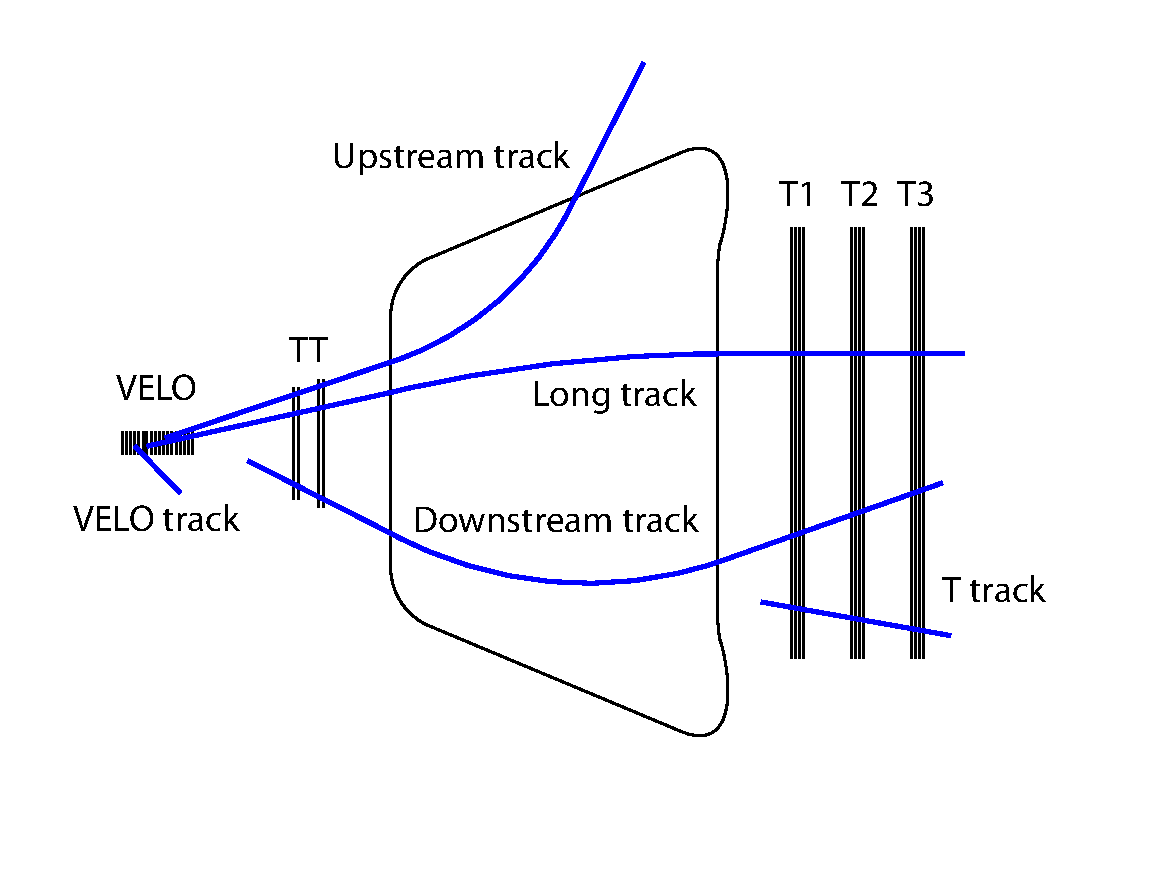
\includegraphics[width=0.7\textwidth]{Figures/Chapter2/trackTypesRunIAndII}
  \caption{\lhcb track types.}
  \label{track_types}
\end{figure}

A charged particle that traverses the \lhcb magnet is deflected. The amount of deflection is inversly proportional
to its momentum. The latter is exploited by tracking algorithms to estimate the momentum of a track. The relative
momentum momentum resolution of the tracking sytem, shown in \figref{det_deltappvp}, is $\nicefrac{\Delta p}{p} = 0.5 \%$
for low mementum tracks and up to $1\%$ at 200\gevc. Intuitively, tracks that do not deflect a lot have inferior momentum
resolution.

Measuring the mass a particle, like the \Bs meson, is achieved by combining tracks in order to build an entire
cascade of partcile decays (or simply decay chanell). The presition on the previous quantities varies depending
on the specific decay chanell. Two body \B decays including a \jpsi have the most precise mass resolution of about
$8 \mevcc$. On the other hand decay chanells including neutral particles, \ie $\Bs\to\phi\gamma$, have a worst resolution of about $100 \mevcc$.

\begin{figure}[t]
  \centering
  \includegraphics[width=0.48\textwidth]{Figures/Chapter2/dppVsp-crop-cmyk}
  \includegraphics[width=0.48\textwidth]{Figures/Chapter2/DataResXY_1PV_2012-crop-cmyk.pdf}
  \caption{\lhcb Momentum resolution and pv resolution.}
  \label{det_deltappvp}
\end{figure}

Certain important analysis performed at \lhcb rely on measuring the {\it flight distance} of a particle, like the \Bs meson.
Flight distance is typically the distance between the point were the two protons colideed, called {\it Primary Vertex} (PV)
and the point were the \Bs, in that case, decaied, called {\it Secondary Vertex} (SV). The \velo sub-detector was designed
for optimum spacial resolution, by placing the \velo sensors as close to the beam as posible. The PV resolution depends
strongly on the number of tracks present in the vertex and can be seen in \figref{}. Measuring the flight distance translates
to a {\it decay time} time measurement. The latter is time interval between the production and the decay of a particle is the
actual quantity that a typical {\it time dependant} analysis requires. The average decay time resolution measured with \BsJpsiPhi
events is $\sim 45\fs$

Lastly, a big part of the \lhcb physics program includes muons. The muon system consit of silicon pads and is placed after
the calorimeters, since the muons can penetrate through a large volume of led without decaying.
Each of the 5 muon stations is sub-devided into in four regions. {\color{red} The M1 muon station not used ??()}
The granularity of each pad size is progresively smaller as one moves closer to the beam pipe. This is done to acount
for the large number of tracks that are found in the forward region and require small pad sizes to keep the number
of ghost hits managable. The overall hit efficiency is above $97\%$.
